
\setcounter{chapter}{2}
\chapter{System Design and Architecture}
\label{ch:system_design}
\minitoc %insert la minitoc
\graphicspath{{Chapitre3/figures/}}

%\DoPToC
%==============================================================================
\pagestyle{fancy}
\fancyhf{}
\fancyhead[R]{\bfseries\rightmark}
\fancyfoot[R]{\thepage}
\renewcommand{\headrulewidth}{0.5pt}
\renewcommand{\footrulewidth}{0pt}
\renewcommand{\chaptermark}[1]{\markboth{{\chaptername~\thechapter. #1 }}{}}
\renewcommand{\sectionmark}[1]{\markright{\thechapter.\thesection~ #1}}

\begin{spacing}{1.2}

%==============================================================================
\section*{Introduction}
This chapter presents the system design and architecture of the LLM-powered best practices enforcement system. Building on the business understanding and requirements established in Chapter 2 ~\ref{ch:business_understanding}, it details technical design decisions, architectural patterns, and system components that enable real-time, intelligent feedback for YouTube framework development.

The design follows traditional software engineering principles while incorporating modern AI technologies. This chapter covers the overall system architecture, component design, data models, and integration patterns that form the foundation of the implemented solution.

\section{System Architecture Overview}

\subsection{High-Level Architecture}
The system architecture is designed to integrate seamlessly into the developer's existing workflow while providing intelligent, context-aware feedback. It consists of two main components:

\begin{itemize}
    \item \textbf{IDE:} The developer's workspace that hosts the YouTube IDE Extension, which serves as the entry point and user‑facing interface. It's a familiar part of YouTube developers' workflow that aims to improve different aspects of the developer experience.
    \item \textbf{AI Agent Framework:} This is the serving infrastructure for LLM-powered applications, or agents developed by YT DevInfra. It aims to make deploying such applications easy by providing out-of-the-box functionality and encouraging reuse of existing LLM libraries. It hosts the LLM Best Practices Agent, which performs code analysis and generates best practice suggestions.
\end{itemize}

\begin{figure}[H]
\centering
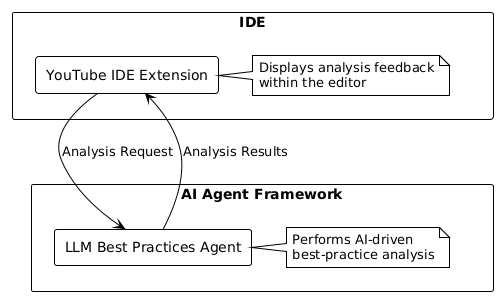
\includegraphics[scale=0.7]{images/high_level_system_architecture.png}
\caption{High-Level System Architecture}
\label{fig:system_architecture}
\end{figure}

Figure~\ref{fig:system_architecture} illustrates the separation between the IDE extension and the AI processing backend. The IDE provides immediate access to analysis capabilities, while the AI Agent Framework handles computationally intensive tasks. This separation allows independent scaling of AI capabilities without impacting IDE responsiveness.

\subsection{System Workflow}
The system operates through a streamlined workflow beginning when a developer triggers analysis via the IDE Extension (Figure~\ref{fig:sequence_diagram}).

\begin{figure}[H]
\centering
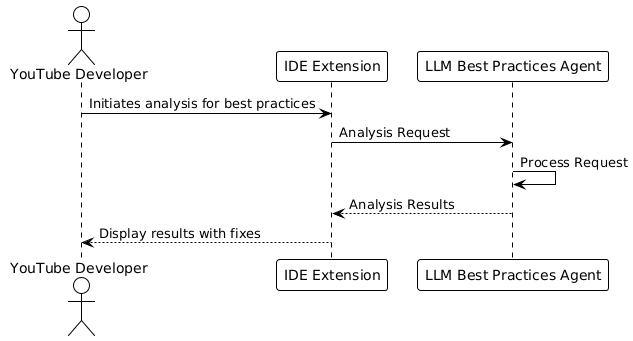
\includegraphics[scale=0.7]{images/sequence_diagram.png}
\caption{System Interaction Sequence Diagram}
\label{fig:sequence_diagram}
\end{figure}

The primary workflow includes:

\begin{enumerate}
    \item \textbf{Analysis Initiation:} The developer triggers analysis on the open file.
    \item \textbf{Request Submission:} The IDE Extension submits the request to the AI agent, identifying the target file.
    \item \textbf{Processing:} The agent performs best-practices analysis.
    \item \textbf{Result Delivery:} The agent returns structured findings.
    \item \textbf{Presentation:} The IDE Extension displays violations and suggested fixes in the editor.
\end{enumerate}

This workflow decouples the IDE from heavy computation, maintaining responsiveness while delegating analysis to the specialized agent framework.

\section{LLM Best Practices Agent}

The LLM Best Practices Agent is the core intelligence engine of the system. Its responsibilities include analyzing code, detecting violations of internal YouTube framework best practices, providing human-readable explanations, and suggesting actionable fixes. This component represents the intersection of AI capabilities with domain-specific software engineering expertise.

\subsection{Core Tools Architecture}
We begin with the building blocks the agent orchestrates. Aligned with the AI agent architecture introduced in Chapter~\ref{ch:business_understanding}, the agent uses specialized tools, each responsible for a specific step of the best practices enforcement pipeline:

\begin{figure}[H]
\centering
\begin{tikzpicture}[>=latex]
  % Central agent
  \node[draw, rounded corners, fill=blue!10, align=center, inner sep=6pt, text width=3.8cm] (agent) {LLM Best Practices Agent\\[2pt]
\includegraphics[width=1.0cm]{images/agent.png}};

  % Tools around in a circle
  \node[draw, rounded corners, align=center, inner sep=4pt, text width=3.8cm] (file) at (90:4.2cm) {\textbf{Tool 1:} File Reading Tool\\[2pt] 
\includegraphics[width=0.9cm]{images/read_file_tool.png}};
  \node[draw, rounded corners, align=center, inner sep=4pt, text width=4.0cm] (analysis) at (18:5.4cm) {\textbf{Tool 2:} Code Analysis Tool\\[2pt] 
\includegraphics[width=0.9cm]{images/code_analysis_tool.png}};
  \node[draw, rounded corners, align=center, inner sep=4pt, text width=4.2cm] (explain) at (-54:4.2cm) {\textbf{Tool 3:} Violation Explanation Tool\\[2pt] 
\includegraphics[width=0.9cm]{images/explanation_tool.png}};
  \node[draw, rounded corners, align=center, inner sep=4pt, text width=3.8cm] (fix) at (-126:4.2cm) {\textbf{Tool 4:} Code Fix Tool\\[2pt]
\includegraphics[width=0.9cm]{images/code_fix_tool.png}};
  \node[draw, rounded corners, align=center, inner sep=4pt, text width=4.2cm] (consolidate) at (162:5.4cm) {\textbf{Tool 5:} Result Consolidation Tool\\[2pt] 
\includegraphics[width=0.9cm]{images/consolidation_tool.png}};

  % Arrows between agent and tools
  \draw[->] (agent) -- (file);
  \draw[->] (file) -- (agent);

  \draw[->] (agent) -- (analysis);
  \draw[->] (analysis) -- (agent);

  \draw[->] (agent) -- (explain);
  \draw[->] (explain) -- (agent);

  \draw[->] (agent) -- (fix);
  \draw[->] (fix) -- (agent);

  \draw[->] (agent) -- (consolidate);
  \draw[->] (consolidate) -- (agent);
\end{tikzpicture}
\caption{The LLM Best Practices Agent orchestrating interactions with its specialized tools}
\label{fig:agent_tools}
\end{figure}

As illustrated in Figure~\ref{fig:agent_tools}, the agent sits at the center and interacts with five specialized tools to complete the analysis. The roles of these tools are summarized below:

\begin{itemize}
    \item \textbf{File Reading Tool:} Retrieves complete file content. Ensures full context for downstream analysis.
    
    \item \textbf{Code Analysis Tool:} Performs structural and semantic analysis against internal framework rules, considering local context around each finding. Combines static analysis heuristics with LLM-based reasoning to flag location, rule identifier, and a short rationale.
    
    \item \textbf{Violation Explanation Tool:} Converts raw violations into human-readable explanations, providing actionable insight and contextual rationale for developers.
    
    \item \textbf{Code Fix Tool:} Suggests concrete, minimal edits that align with framework conventions. Generates patch‑style suggestions or structured steps to help developers resolve the violation confidently.
    
    \item \textbf{Result Consolidation Tool:} Aggregates outputs from all tools into a structured response consumable by the IDE extension, ensuring clear and contextually accurate presentation.
\end{itemize}

\subsection{Integration with LLM Infrastructure}
With tool responsibilities defined, the agent interfaces with an internal AI platform hosting multiple LLM models. Key design considerations include:

\begin{itemize}
    \item \textbf{Model-Agnostic Orchestration:} The architecture supports seamless adoption of new models without modifying the agent workflow.
    \item \textbf{Stable Interfaces:} Each tool interacts with the LLM via encapsulated, stable APIs to ensure maintainability.
\end{itemize}

\subsection{Agent Architecture Options}
Now that the tools are defined, the question is how the agent will orchestrate them. We consider two agent architecture options our internal AI Agent Framework offers: Executable and ReAct. We explored these paradigms for the agent, drawing inspiration from established AI agent patterns~\cite{microsoftAgentPatterns}. Figure~\ref{fig:agent_comparison} illustrates the fundamental differences in control flow between these two options.

\begin{figure}[H] 
    \centering 
    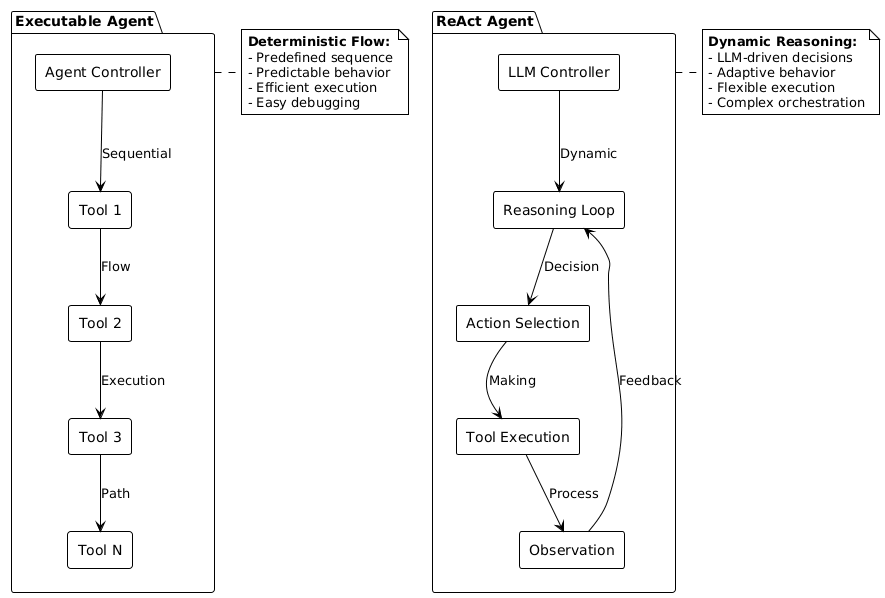
\includegraphics[scale=0.6]{images/agent_architecture_comparison.png} 
    \caption{Comparison of Executable Agent vs. ReAct Agent Architectures} 
    \label{fig:agent_comparison} 
\end{figure}

\begin{itemize}
    \item \textbf{ReAct Agent:} Integrates \emph{reasoning and acting} in a closed loop. The agent interprets the goal, plans the next step, selects and invokes a tool, observes the result, and updates its internal trace before continuing. This iterative control flow supports open‑ended problem solving, dynamic tool chaining, and exploratory analysis. ReAct agents typically maintain a short‑term action log (thoughts, tool calls, observations) that explains how outcomes were reached and can be surfaced as an execution trace for review.
    
    \item \textbf{Executable Agent:} Encodes a deterministic, predefined workflow as an explicit sequence or graph of steps. Each step is a well‑typed tool or validator with clearly defined inputs, outputs, and pre/post‑conditions, and the LLM is invoked within steps for domain‑specific processing rather than global orchestration. This structure enables precise routing, step‑level retries and fallbacks, policy gates, and comprehensive telemetry at each stage, making execution easy to audit, measure, and operate at scale.
\end{itemize}

\subsection{Processing Strategy Options}
Complementing these architecture options, the processing strategy governs how the agent sequences and (when appropriate) parallelizes analysis across findings. It directly impacts IDE responsiveness, determinism, and operational cost. In our setting, a single file may surface many candidate violations; to handle this efficiently and predictably, we considered three strategies:

\begin{itemize}
    \item \textbf{Fully Sequential:} Processes one finding at a time in a clear, step‑by‑step flow. Each finding is analyzed, optionally fixed, and then the next one is handled. This makes the execution easy to follow and the output straightforward to review.
    
    \item \textbf{Fully Parallel:} Processes all findings at once. The agent analyzes each finding independently and then returns a single, consolidated result. This mode is suited to fast, whole‑file scans and bulk reporting.
    
    \item \textbf{Hybrid Approach:} Processes a small set of findings together, then moves on to the next set. It combines the readability of sequential steps with the speed of parallel checks, keeping the experience smooth for larger files.
\end{itemize}

\section{Evaluation Framework for Architecture Decisions}
Given the complexity and multiple viable options for agent architecture and processing strategies, empirical evaluation is essential. Decisions cannot be based solely on intuition; performance, reliability, and quality need to be measured under realistic conditions.

We consider three candidates:

\begin{itemize}
    \item \textbf{Sequential Executable Agent}
    \item \textbf{Parallel Executable Agent}
    \item \textbf{ReAct Agent}
\end{itemize}

\subsection{Test Suite Framework}
We selected a set of 12 diverse source files. For each file, we manually reviewed the code to identify violations, then defined evaluation cases with expected outcomes: findings, explanations, and minimal fixes. This provides a reproducible ground truth and enables fair comparisons across runs.

\paragraph{Coverage dimensions}
\begin{itemize}
    \item \textbf{File size and structure}: small, medium, and large files.
    \item \textbf{Violation density}: none (clean baselines), sparse, dense, and clustered violations.
    \item \textbf{Pattern complexity}: straightforward single‑line issues vs. multi‑line, context‑dependent patterns.
    \item \textbf{Error‑inducing cases}: inputs designed to trigger errors or timeouts to validate failure handling and recovery.
    \item \textbf{Rule categories}: naming/structure, lifecycle/ordering, performance‑sensitive conventions, and readability/documentation.
    \item \textbf{Conflict/overlap}: cases where multiple rules trigger on the same span or produce competing suggestions.
    \item \textbf{Language constructs}: different control‑flow forms, data structures, and API usages.
\end{itemize}


\subsection{LLM-as-a-Judge Methodology}
Each evaluation case specifies an expected output (gold findings, explanations, and minimal fixes). Direct string comparison is brittle: semantically correct answers may differ in phrasing, ordering, or formatting. To compare the agent output to the gold robustly, we use an independent \textbf{\emph{LLM-as-a-Judge}} that evaluates semantic equivalence and quality.

\begin{figure}[H]
\centering
\begin{tikzpicture}[>=latex]
  % Nodes
  \node[draw, rounded corners, align=center, inner sep=6pt, text width=4.0cm] (gold) {Expected Output\\(gold, hard-coded)\\[2pt]
\includegraphics[width=0.9cm]{images/gold_truth.png}};
  \node[draw, rounded corners, align=center, inner sep=6pt, text width=4.0cm] (agentout) at (0,-3.2) {Agent Output\\(LLM-generated)\\[2pt]
\includegraphics[width=1cm]{images/llm_generated.png}};
  \node[draw, rounded corners, fill=blue!10, align=center, inner sep=6pt, text width=4.4cm] (judge) at (6.2,-1.1) {LLM as a Judge\\[2pt]
\includegraphics[width=1.5cm]{images/llm_judge.png}};
  \node[draw, rounded corners, align=center, inner sep=6pt, text width=4.4cm] (result) at (12.4,-1.1) {Score + Reasoning\\(pass/fail, justification)\\[2pt]
\includegraphics[width=1.1cm]{images/speedometer.png}};

  % Arrows
  \draw[->] (gold) -- (judge);
  \draw[->] (agentout) -- (judge);
  \draw[->] (judge) -- (result);
\end{tikzpicture}
\caption{LLM-as-a-Judge}
\label{fig:llm_judge_flow}
\end{figure}

LLM-as-a-Judge is an evaluation paradigm in which a separate LLM grades model outputs against a reference (gold) or via pairwise comparison using an explicit rubric, then returns a score and brief rationale; prior work reports strong correlation with expert human judgments when prompts and rubrics are well specified~\cite{zheng2023judging}.

In our evaluation, we use a \textbf{rubric‑based, reference comparison}. “Rubric‑based” means the judge applies a small, explicit checklist of acceptance criteria; “reference comparison” means the agent output is evaluated against a hand‑labeled gold reference rather than another model output. The judge compares the agent output to the gold reference and returns a pass/fail decision with a brief rationale.

Rubric (acceptance criteria):
\begin{itemize}
    \item Missing any expected convention \textrightarrow{} fail
    \item Hallucinated/extra conventions not in gold \textrightarrow{} fail
    \item Ordering differences do not matter
    \item Values/ranges must match within a small tolerance (e.g., ±10\%)
    \item Returned an error for a case where a valid answer exists \textrightarrow{} fail
    \item Explanations and suggested fixes must be consistent with the referenced convention and not contradict gold
    \item Formatting differences are ignored unless they change meaning
\end{itemize}

\noindent A case passes only if all rubric criteria are satisfied; any unmet criterion results in a fail.

\subsection{Key Metrics}
The evaluation framework measures three primary dimensions:

\begin{itemize}
    \item \textbf{Accuracy:} Semantic correctness of analysis results and suggested fixes, as judged by the LLM evaluator.
    \item \textbf{Latency:} End-to-end response time, ensuring real-time usability in the IDE.
    \item \textbf{Cost:} Token consumption, API usage, and compute resource requirements.
\end{itemize}

Each agent architecture option is assessed using the test suite and the LLM-as-a-Judge methodology, producing data-driven insights into trade-offs between determinism, throughput, accuracy, and operational cost. This combination of structured evaluation and modular design ensures that architecture and processing strategies can be selected with confidence, balancing performance, reliability, maintainability, and developer usability.


\section{YouTube IDE Extension Integration}
As introduced above, the YouTube IDE Extension is the user‑facing interface that integrates analysis into developers' daily workflow. This section details its architecture and interaction patterns, focusing on in‑editor, context‑aware feedback while preserving IDE responsiveness.

\subsection{Extension Architecture}
The YouTube IDE Extension serves as \textbf{a lightweight client} that orchestrates the interaction between developers and the AI analysis system. The architecture ensures responsiveness by delegating computationally intensive analysis to the specialized agent framework while handling user interface concerns, progress indication, and result presentation locally.

\subsection{User-Triggered vs. Automatic Analysis}
A fundamental design decision for the IDE extension was whether to implement user-triggered analysis or automatic analysis. This choice significantly impacts user experience, system performance, and resource utilization.

The primary motivation for user-triggered analysis stems from the need to maintain developer productivity and system efficiency. \textbf{LLM analysis} is computationally expensive and resource-intensive, making continuous analysis impractical for maintaining IDE responsiveness. \textbf{User-triggered analysis} ensures that analysis occurs only when developers specifically request it, providing contextually relevant feedback at optimal moments without interrupting their workflow. This approach aligns with developer expectations of having control over their development environment while ensuring that computational resources are used efficiently.

Table~\ref{tab:analysis_approaches} summarizes the comparison of user-triggered vs. automatic analysis approaches:

\begin{table}[H]
\centering
\caption{Comparison of User-Triggered vs. Automatic Analysis Approaches}
\label{tab:analysis_approaches}
\begin{tabular}{|l|c|c|}
\hline
\textbf{Criteria} & \textbf{User-Triggered} & \textbf{Automatic} \\
\hline
User Control & $\checkmark$ & $\times$ \\
\hline
Resource Efficiency & $\checkmark$ & $\times$ \\
\hline
IDE Performance & $\checkmark$ & $\times$ \\
\hline
Contextual Timing & $\checkmark$ & $\times$ \\
\hline
Discoverability & $\times$ & $\checkmark$ \\
\hline
Always Current & $\times$ & $\checkmark$ \\
\hline
\end{tabular}
\end{table}

Based on this analysis, \textbf{the user-triggered approach was selected} as it provides superior resource management, user control, and system performance. The trade-offs in discoverability and stale state management are addressed through intuitive UI design and comprehensive feedback mechanisms.

\paragraph{Stale State Challenge}
The user-triggered approach introduces a fundamental design challenge: maintaining the relevance and accuracy of analysis results as developers continue modifying their code. This challenge requires balancing system responsiveness with result accuracy, ensuring that feedback remains useful throughout the development process.

\subsection{User Interface Design}
The YouTube IDE Extension is designed around two core interaction patterns: entry points for initiating analysis and feedback mechanisms for presenting results.

\paragraph{Entry Points}
The YouTube IDE Extension provides multiple entry points to ensure accessibility and discoverability for different user preferences and workflows:

\begin{itemize}
    \item \textbf{Visual Interface Integration}: Visual indicators are integrated into the development environment to provide immediate visibility of AI analysis availability, ensuring maximum discoverability while maintaining a clean interface.
    
    \item \textbf{Command-Based Access}: For developers who prefer keyboard-driven workflows, the extension provides command-based access through standard IDE navigation patterns, supporting both mouse-driven and keyboard-driven user interactions.
\end{itemize}

\paragraph{Feedback Mechanisms}
The YouTube IDE Extension employs three core feedback mechanisms designed to integrate seamlessly with existing development workflows:

\begin{itemize}
    \item \textbf{Progress Indication}: Real-time status updates during analysis processing to maintain developer awareness and system transparency.
    
    \item \textbf{Violation Display}: Presentation of analysis results using familiar interface patterns that leverage developers' existing knowledge of standard feedback mechanisms.
    
    \item \textbf{Contextual Suggestions}: Interactive code solutions that appear when developers interact with violation markers, providing actionable recommendations.
\end{itemize}


\subsection{User Interaction Flow}
The user interaction flow with the YouTube IDE Extension follows a structured pattern from analysis initiation to optional fix application:

\begin{figure}[H]
\centering
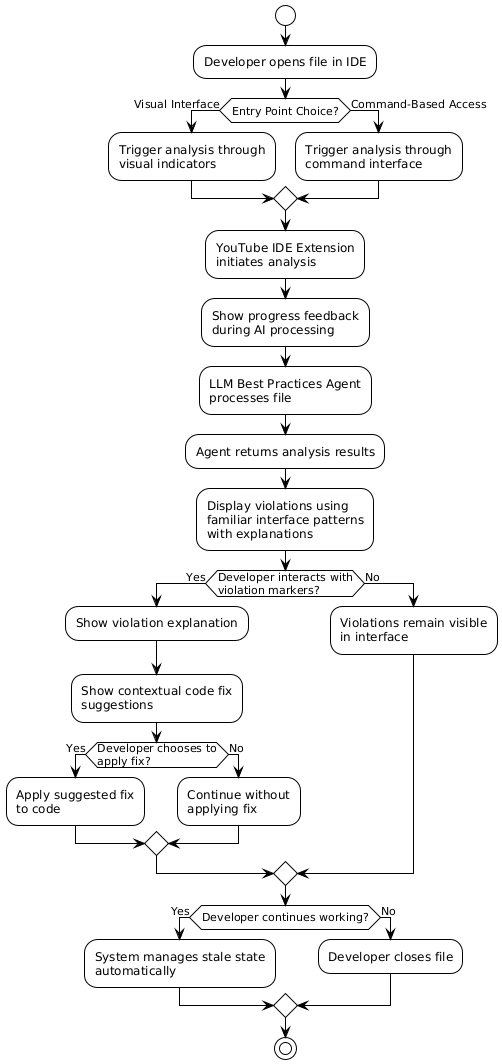
\includegraphics[scale=0.6]{images/user_flow.png}
\caption{YouTube IDE Extension User Interaction Flow: Complete developer journey from analysis trigger to fix application}
\label{fig:user_interface_flow}
\end{figure}

As illustrated in Figure~\ref{fig:user_interface_flow}, the flow demonstrates the core interaction pattern: developers initiate analysis through visual or command interfaces, receive progress feedback during processing, and interact with displayed violations to access explanations and optional fixes. This design ensures developers maintain control over their workflow while providing comprehensive feedback when requested.


\section{Data Models and Interfaces}

\subsection{Input/Output Specification}
The system's data models define the contracts between components, ensuring consistent communication and data exchange throughout the analysis pipeline. These interfaces establish clear boundaries between the IDE extension and the AI agent, enabling independent evolution of each component.

\paragraph{Analysis Request Format}
The YouTube IDE Extension sends analysis requests to the LLM Best Practices Agent using a minimal input format that identifies the target file for analysis. This design choice ensures that the agent can focus on its core responsibility of code analysis while maintaining security and proper workspace isolation. The request format includes the file path.

\paragraph{Analysis Response Format}
The agent returns a structured response containing the analysis results, error information, and optional metadata. The response format includes status information indicating success or failure, violation details with explanations and suggested fixes, and usage statistics for monitoring purposes. This standardized format ensures that the IDE extension can consistently process and display results regardless of the underlying analysis complexity.

\subsection{Convention Data Management}
The system's convention data model defines how YouTube framework best practices are structured, stored, and accessed throughout the analysis pipeline.

\paragraph{Convention Data Structure}
The convention data model captures best practice definitions as structured objects that support efficient programmatic access and analysis. Each convention definition includes essential metadata such as unique identifiers, descriptions, correct examples, and incorrect examples. This structure enables rapid lookup and context-specific retrieval during code analysis, with the design optimized for constant-time access patterns required by the agent's processing pipeline.

\paragraph{Storage Architecture Decision}
The system employs an in-memory storage approach using structured objects rather than external file-based or database storage. This design decision balances several architectural considerations:

\begin{itemize}
    \item \textbf{Data Characteristics}: Conventions are static during runtime, requiring no dynamic updates, making in-memory storage appropriate for performance-critical analysis.
    \item \textbf{Performance Requirements}: In-memory access ensures ultra-low-latency retrieval for real-time analysis, eliminating I/O overhead during agent execution.
    \item \textbf{Simplicity \& Reliability}: Structured objects provide type safety and eliminate parsing overhead while ensuring data integrity.
    \item \textbf{Resource Efficiency}: Conventions are loaded once at startup, minimizing runtime resource consumption and avoiding repeated file system access.
    \item \textbf{Architectural Flexibility}: The design allows future migration to external storage if multi-framework support or dynamic updates become necessary.
\end{itemize} 

\paragraph{Integration Interfaces}
The system defines minimal, versioned boundaries that keep components decoupled:

\begin{itemize}
    \item \textbf{IDE Extension Interface}: Contract between the YouTube IDE Extension and the LLM Best Practices Agent that defines the analysis request and response format, enabling independent evolution of UI and agent components.
    \item \textbf{Convention Access Interface}: Defines how the agent accesses convention definitions through in-memory lookup mechanisms, providing a stable boundary for data retrieval without external dependencies.
    \item \textbf{Monitoring Interface}: Captures usage statistics and performance metrics for system observability and evaluation purposes.
\end{itemize}


\subsection*{Conclusion}
This chapter defined the end‑to‑end design of the system: a high‑level architecture that separates the IDE extension from the AI backend; the LLM Best Practices Agent with its core tools and model integration; alternative agent architectures and processing strategies; a pragmatic evaluation framework leveraging a rubric‑based LLM‑as‑a‑Judge; and the IDE integration and data contracts that make the experience usable in practice. Together, these elements provide a clear, modular foundation for enforcing framework best practices with AI, while enabling data‑driven selection among viable execution options. The next chapter turns to implementation details and empirical results based on this design.
%==============================================================================
\end{spacing}
